%% distro.tex
%% Copyright 2015 Gaël PORTAY <gael.portay@gmail.com>
%
% This work may be distributed and/or modified under the
% conditions of the LaTeX Project Public License, either version 1.3
% of this license or (at your option) any later version.
% The latest version of this license is in
%   http://www.latex-project.org/lppl.txt
% and version 1.3 or later is part of all distributions of LaTeX
% version 2005/12/01 or later.
%
% This work has the LPPL maintenance status `maintained'.
%
% The Current Maintainer of this work is Gaël PORTAY.
%
% This work consists of the file distro.tex.

\documentclass[a4paper]{article}
\usepackage{caption}
\usepackage{graphicx}
\usepackage{hyperref}
\usepackage{listings}
\usepackage[T1]{fontenc}
\usepackage[utf8]{inputenc}
\usepackage[francais]{babel}

\lstloadlanguages{[ANSI]C,sh,make}

\title{Ma première distribution Linux faite maison}
\author{Gaël PORTAY}
\date{\today}

\begin{document}
\sloppy
\maketitle

\tableofcontents

\clearpage
\part{Le noyau}

\section{Première compilation}

Entrons directement dans le vif du sujet et attaquons par la compilation d'un noyau \textit{Linux} ! Nous allons compiler un noyau pour l'architecture hôte : la machine sur laquelle vous travaillez actuellement\footnote{Dans un premier temps, je supposerai que vous travaillez sur une machine à base de processeur \textit{Intel x86}. Les extraits de code disponibles à travers ce document sont donnés pour cette architecture. Si vous travaillez sur une autre architecture (exemple : \textit{PowerPC} (\textit{PPC})), vous devrez adapter ces extraits pour votre machine. J'adapterai ces extraits plus tard pour qu'ils soient génériques et puissent être utilisés sur n'importe quelle architecture.}.\\

Je n'aborderai pas ici les concepts de la \textit{compilation croisée}. «~La compilation quoi ?!? croisée ?!?~». Hum... le plus simple est de consulter la page \textit{Wikipédia} sur la \textit{compilation croisée}\footnote{\url{https://fr.wikipedia.org/wiki/Compilateur\#Compilation\_crois.C3.A9e}}. Grosso modo, on compile un programme destiné à être exécuté sur une architecture cible autre que l'architecture hôte, celle sur laquelle on est entrain de compiler. Vous n'y êtes toujours pas ?!? Plus simplement, on compile quelque-chose sur notre \textit{PC} à base de processeur \textit{Intel} (\textit{x86}) destiné à être utilisé sur un \textit{Raspberry-PI} (\textit{ARM}). C'est bon vous y êtes ?!? Avec un exemple c'est toujours plus facile à comprendre...\\

Vous êtes prêts ?!? Alors c'est parti !\\

\subsection{Les fichiers sources}

Nous allons avoir besoin des fichiers sources de \textit{Linux}. Pour cela, rien de plus simple : allons sur le site \href{http://www.kernel.org}{kernel.org} pour télécharger la dernière version stable\footnote{A l'heure où j'écris ces lignes, la dernière version stable est la version 4.3.}.\\

La règle \textit{Makefile}, ci-dessous, automatise le téléchargement et le désarchivage de la dernière version stable. Vous pouvez la réutiliser en effectuant un copier/coller dans un fichier \textit{Makefile} et ensuite exécuter la commande suivante : \lstset{language=sh}\lstinline{make linux_download}.\\

\lstset{language=make}
\lstinputlisting[firstline=32,lastline=35,breaklines]{../kernel/Makefile}

Pour le reste de ce document, nous supposerons que les fichiers sources sont dans le répertoire \textbf{./linux}.\\

\subsection{make}

Nous y voilà, nous sommes fin prêts pour compiler notre premier noyau ! Excité, non ?!? Allez, on est parti. Ouvrez un terminal (si ce n'est pas déjà fait) et lancez la commande : \lstset{language=sh}\lstinline{cd linux && make} et...

\begin{verbatim}
$ make
  HOSTCC  scripts/basic/fixdep
  HOSTCC  scripts/kconfig/conf.o
  SHIPPED scripts/kconfig/zconf.tab.c
  SHIPPED scripts/kconfig/zconf.lex.c
  SHIPPED scripts/kconfig/zconf.hash.c
  HOSTCC  scripts/kconfig/zconf.tab.o
  HOSTLD  scripts/kconfig/conf
scripts/kconfig/conf  --silentoldconfig Kconfig
***
*** Configuration file ".config" not found!
***
*** Please run some configurator (e.g. "make oldconfig" or
*** "make menuconfig" or "make xconfig").
***
scripts/kconfig/Makefile:37: recipe for target 'silentoldconfig' failed
make[2]: *** [silentoldconfig] Error 1
Makefile:531: recipe for target 'silentoldconfig' failed
make[1]: *** [silentoldconfig] Error 2
  SYSTBL  arch/x86/entry/syscalls/../../include/generated/asm/syscalls_32.h
  SYSHDR  arch/x86/entry/syscalls/../../include/generated/uapi/asm/unistd_32.h
  SYSHDR  arch/x86/entry/syscalls/../../include/generated/uapi/asm/unistd_64.h
  SYSHDR  arch/x86/entry/syscalls/../../include/generated/uapi/asm/unistd_x32.h
  HOSTCC  arch/x86/tools/relocs_32.o
  HOSTCC  arch/x86/tools/relocs_64.o
  HOSTCC  arch/x86/tools/relocs_common.o
  HOSTLD  arch/x86/tools/relocs
make: *** No rule to make target 'include/config/auto.conf', needed by 'include/config/kernel.release'.  Stop.
\end{verbatim}

C'était trop beau pour être vrai... compiler son noyau n'est pas aussi simple ! \textit{Linux} est une noyau \textit{monolithique} \textit{modulaire} qui supporte plusieurs \textit{architectures} (promis, je ne voulais pas offenser). Comprenez simplement que le projet a besoin d'être configuré avant de pouvoir être compilé avec un vulgaire \lstset{language=sh}\lstinline{make}.\\

\clearpage
\section{Configuration}

\textit{Linux} utilise le langage \textit{\href{https://www.kernel.org/doc/Documentation/kbuild/kconfig-language.txt}{Kconfig}} pour décrire ses options de configurations. Ces options sont définies dans les fichiers \textbf{Kconfig}. Ils sont présents un peu partout dans les répertoires des fichiers sources, à l'image des \textit{Makefiles}.\\

Il existe plusieurs \textit{front-ends} (interfaces) pour afficher le menu de configuration du noyau. Généralement, les développeurs (ou «~Kernel Hackers~») utilisent la bonne vielle interface en \textit{ncurses}, invoquée via le \textit{Makefile} et sa règle \textbf{menuconfig} (\lstset{language=sh}\lstinline{make menuconfig}). Il existe également d'autres interfaces comme \textbf{config} (en ligne de commande), \textbf{nconfig} (nouvelle interface \textit{ncurses}), \textbf{xconfig} (interface \textit{Qt}) et \textbf{gconfig} (interface \textit{GTK+}).\\

Revenons à nos moutons... Lorsque notre première commande \lstset{language=sh}\lstinline{make} a échouée, vous avez sûrement remarqué le message suivant :
\begin{verbatim}
***
*** Configuration file ".config" not found!
***
*** Please run some configurator (e.g. "make oldconfig" or
*** "make menuconfig" or "make xconfig").
***
\end{verbatim}

Le fichier \textbf{.config} est manquant ! Ce fichier contient la configuration du noyau. C'est une simple liste des options qui seront compilées ou non, intégrées à l'image du noyau ou disponibles via un module.\\

Bien entendu, les sources du noyau viennent sans aucune configuration. Nous allons donc devoir générer cette configuration.\\

\subsection{menuconfig}

Allez, on se fait une petite frayeur : configurons notre noyau en exécutant la commande \lstinline{make menuconfig}\footnote{Nous allons avoir besoin du paquet de développement de \textit{ncurses}. Si vous n'y arrivez pas, passez simplement cette partie, elle n'est pas essentielle}.\\

\begin{figure}
\label{fig:make_menuconfig}
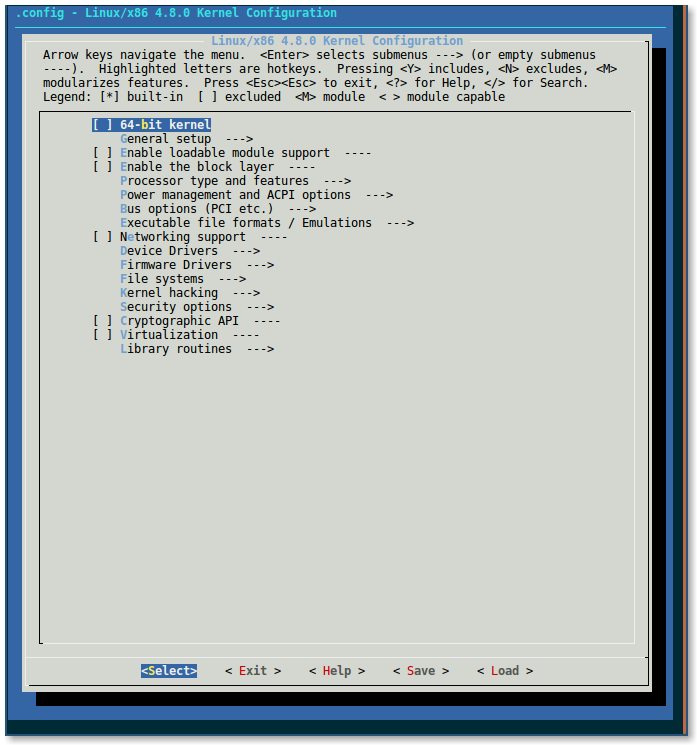
\includegraphics[scale=0.5]{../res/make-menuconfig.png}
\caption{make menuconfig}
\end{figure}

La figure~\ref{fig:make_menuconfig} montre le menu principal de configuration du noyau. Vous pouvez vous balader dans les sous-menus avec les flèches \textit{haut} et \textit{bas} ; entrer dans les sous-menu avec la touche \textit{Entrée} ; retourner au menu précédent avec la touche \textit{Échap} ; cocher/décocher les options avec la touche \textit{Espace}. Maintenant, quittez sans sauvegarder \textit{Ctrl-C} et \textit{No}\footnote{Si vous avez malencontreusement sauvegardé, supprimez le fichier \textbf{.config} via \lstset{language=sh}\lstinline{rm .config}}.\\

Vous l'aurez vite compris, le noyau contient des milliers d'options et donc un nombre incalculable de configurations possibles ! Comment allons-nous configurer notre noyau ?!? Quels sont les pilotes (\textit{drivers}) que nous devons compiler ?!?

\subsection{tinyconfig}

Nous allons créer une configuration minimale du noyau. Pour cela, nous invoquons la règle \textbf{tinyconfig}.

\begin{verbatim}
$ make tinyconfig
scripts/kconfig/conf  --allnoconfig Kconfig
#
# configuration written to .config
#
Using .config as base
Merging ./kernel/configs/tiny.config
Value of CONFIG_CC_OPTIMIZE_FOR_SIZE is redefined by fragment ./kernel/configs/tiny.config:
Previous value: # CONFIG_CC_OPTIMIZE_FOR_SIZE is not set
New value: CONFIG_CC_OPTIMIZE_FOR_SIZE=y
(...)
*
#
# configuration written to .config
#
\end{verbatim}

Le noyau est maintenant configuré ! Un fichier \textbf{.config} est créé à la racine du projet. Ce fichier contient une configuration strictement minimale du noyau.

\section{Compilation}

Voilà, cette fois-ci c'est la bonne : nous sommes parés à compiler notre noyau. Invoquons \lstset{language=sh}\lstinline{make} :\\

\begin{verbatim}
$ make
  GEN     ./Makefile
scripts/kconfig/conf  --silentoldconfig Kconfig
  SYSTBL  arch/x86/entry/syscalls/../../include/generated/asm/syscalls_32.h
  SYSHDR  arch/x86/entry/syscalls/../../include/generated/uapi/asm/unistd_32.h
  SYSHDR  arch/x86/entry/syscalls/../../include/generated/uapi/asm/unistd_64.h
  SYSHDR  arch/x86/entry/syscalls/../../include/generated/uapi/asm/unistd_x32.h
  HOSTCC  arch/x86/tools/relocs_32.o
  HOSTCC  arch/x86/tools/relocs_64.o
  HOSTCC  arch/x86/tools/relocs_common.o
  HOSTLD  arch/x86/tools/relocs
  CHK     include/config/kernel.release
  UPD     include/config/kernel.release
(...)
  LD      arch/x86/boot/setup.elf
  OBJCOPY arch/x86/boot/setup.bin
  OBJCOPY arch/x86/boot/vmlinux.bin
  HOSTCC  arch/x86/boot/tools/build
  BUILD   arch/x86/boot/bzImage
Setup is 15452 bytes (padded to 15872 bytes).
System is 342 kB
CRC 61bf4503
Kernel: arch/x86/boot/bzImage is ready  (#1)
\end{verbatim}

Notre tout premier noyau est disponible là : \textbf{arch/x86/boot/bzImage}.

\clearpage
\listoffigures

\end{document}
